\subsection{High-Pressure Systems}
Anticyclones are meteorological high-pressure systems in which air sinks toward the ground, creating high pressure \cite{spiridonovCyclonesAnticyclonesSpringerLink2020}. This occurs due to the convergence of air from all directions at high altitudes, which forces the air to move downward. The descending air undergoes adiabatic compression, resulting in an increase in the energy of the air molecules, or, in other words, a higher temperature. This rise in energy inhibits cloud formation, as warmer air can hold more moisture. The absence of clouds allows solar radiation to significantly impact the temperature during an anticyclone. Consequently, this leads to a large temperature difference between day and night, with summer anticyclones being associated with high temperatures and winter anticyclones with low temperatures. 

Under normal conditions, the temperature of the air in the atmosphere decreases with the altitude, due to the adiabatic expansion of the air. The cooling per altitude is called the environmental lapse rate and makes it possible for vertical wind movement to occur, when a slight imbalance is introduced to the system. During an anticyclone, adiabatic compression of the air occurs as the air descends. This increases the temperature at lower altitudes. However, this downward movement of air does not reach the ground due to the friction opposed by buildings, forests, valleys, and other obstacles that create friction by disrupting the airflow. Thus, the downward draught will spread out a few hundred meters above the ground and not mix with the air that lies closest to the ground. Since the air closest to the ground remains cool, while the air a few hundred meters up is warmer from the adiabatic compression, an inversion of the environmental lapse rate will be created. This process is called a subsidence inversion and will prevent air mixing between the ground level and the upper layers of the atmosphere \cite{gramschInfluenceSurfaceSubsidence2014}. The temperature profile due to the subsidence inversion can be seen in \autoref{fig:Subsidence_inverion}. 


\begin{figure}[H]
    \centering
    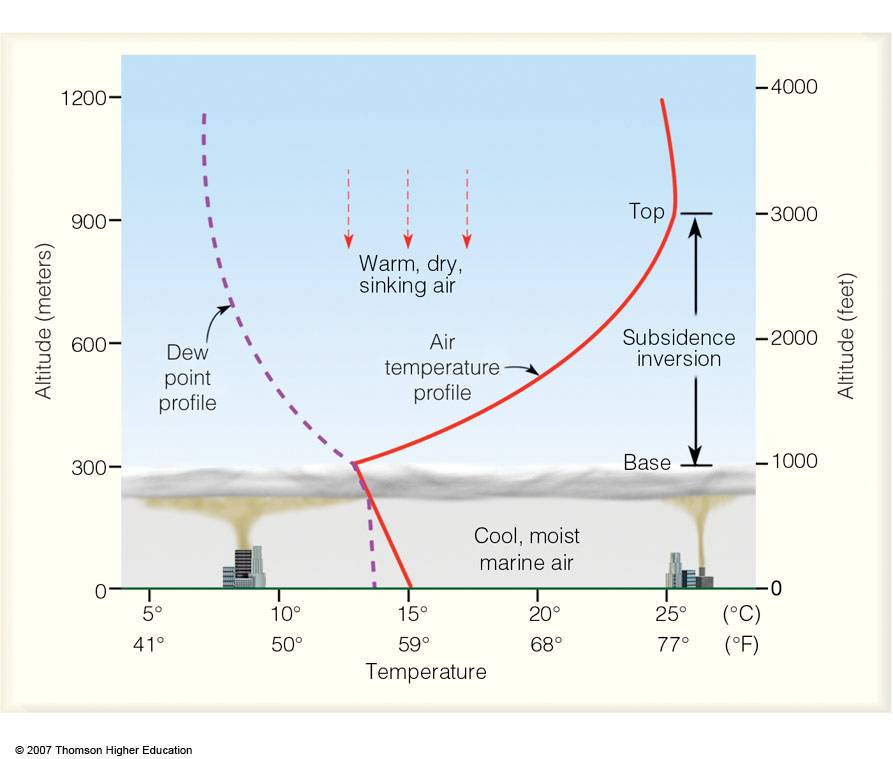
\includegraphics[width=0.55\textwidth]{Figures/subsid_inv_schem.jpg}
    \caption{This figure shows how the temperature changes with altitude under a subsidence inversion in the atmosphere \cite{FormationSubsidenceInversions}.}
    \label{fig:Subsidence_inverion}
\end{figure}

 Another type of inversion occurs during the night as the air closer to the ground loses heat due to the outgoing radiation from the Earth. This process is especially strong due to the absence of clouds during the anticyclone. This creates a ground inversion layer, where the air temperature increases with height closer to the surface \cite{gregohareWeatherClimateClimate2005}. This ground inversion, created from the daily cycle, also prohibits vertical air movement in the atmosphere.

A high-pressure blocking period refers to a prolonged anticyclone characterized by higher surface pressure covering a large area \cite{lupoAtmosphericBlockingEvents2020}. Since the blocking event extends over a vast region, the pressure gradient remains small due to minimal fluctuations. As a result, the wind tends to be calm. A blocking period is typically defined as lasting between five and ten days, although some events can persist even longer \cite{porebskaAnalysisExtremeTemperature2013}. However, no single definition of high-pressure blocking events exists \cite{lupoAtmosphericBlockingEvents2020}. An interesting observation is that the end of a high-pressure blocking event is followed by rainfall and or a strong shift in wind direction. While the concept has been recognized in meteorology for over a century, the long-term consequences of blocking events are not yet fully understood. High-pressure blocking periods are more common in the Northern Hemisphere compared to the Southern Hemisphere. Research has indicated that the frequency of blocking periods has increased in recent years \cite{lupoAtmosphericBlockingEvents2020}. 

Recurring anticyclones can be classified into Hess and Brezowsky macrocirculation types, such as the Fennoscandian High (HFA), the Southeast Anticyclone (SEA), and the Central European High (HM) \cite{bartholyEuropeanCycloneTrack2006}. HFA is centred on the Fennoscandinavian Peninsula (Norway, Sweden, Finland, and western parts of Russia) and is a recurring anticyclone during the winter. This anticyclone is known for blocking air masses from the Atlantic, causing colder periods in the region. The SEA is a recurring anticyclone with its geographical center in southeastern Europe (the Balkans and western Türkiye). This anticyclone is most frequent during the summer months and is associated with heat waves. The HM is centred in central Europe (Germany, Poland, the Czech Republic) and occurs during both the summer and winter months. The center of these anticyclones can be seen in \autoref{fig:map}. 

To explain the air movement during an anticyclone the Navier-Stokes equation can be used,
\begin{equation} 
    \frac{\partial \vec{v}}{\partial t} + (\vec{v} \cdot \nabla)\vec{v} = \vec{g} - \frac{\nabla p}{\rho} - 2\left(\vec{\Omega} \times \vec{v}\right). \label{eq:NavierStokes} 
\end{equation}
The first term in the Navier-Stokes equation corresponds to the local acceleration of the air, the second term corresponds to the convective acceleration of the air, the third term is simply the gravitational acceleration, the fourth term describes the force from the pressure gradient and the last term describes the Coriolis force. Since the aim is to examine the stable solution of this equation, we can assume that the local acceleration is zero. The weather system is a large scale system with the size of hundreds of kilometres, the speed is in the tens of meters per second and the Coriolis term is in the order of \SI{0.5e-4}{\per\s}. Using this information one can observe that the size of the convection term is negligible in comparison to the Coriolis term. Lastly, one can assume the wind to be in the horizontal plane since vertical movement is a lot slower, providing a definition of the wind vector as $\vec{v}=(v_x,v_y,0)$. The Coriolis term can be approximated by considering only the vertical component as $\vec{\Omega}=(0,0,\Omega_z)$, since the horizontal components are negligible and Earth's rotation primarily projects along the vertical axis, causing deflections in the horizontal plane. The Navier-Stokes equation is thus simplified in the case of a stable large scale weather systems to
\begin{equation} 
    0 = - \frac{\nabla p}{\rho} - 2{\vec{\Omega}} \times \vec{v}, \label{eq:NavierStokes2} 
\end{equation}
where the gravity is neglected since it lies in the vertical plane while the wind lies in the horizontal plane. Solving for the horizontal velocity components from this equation one obtains the solution
\begin{equation} v_x=-\frac{1}{2\rho\Omega_z}\frac{\partial p}{\partial y}\text{ and }v_y=\frac{1}{2\rho\Omega_z}\frac{\partial p}{\partial x}. 
\end{equation}
Examining the vorticity of the horizontal wind, one obtains  
\begin{equation}
    (\nabla \times \vec{v})_z  = \frac{1}{2\Omega_z\rho}\nabla^2p,
\end{equation} 
where the definition of the anticyclone (the pressure is strongest in the center) implies that $\nabla^2p$ is negative. Since $\nabla^2p$ is negative the vorticity is also negative, implying that the anticyclone rotates clockwise in the Northern Hemisphere. Since anticyclones exhibit winds rotating clockwise around their center, the winds from HFA, SEA, and HM tend to blow toward southern Sweden from the south, east and west, as can be seen in \autoref{fig:map}. The transport of airborne pollutants, such as ozone, can occur via these winds \cite{oteroImpactAtmosphericBlocking2022}. Consequently, it can be hypothesized that other airborne aerosols, such as \PM, should also be transported through these wind patterns.

\vspace{1cm}

\begin{figure}[H]
    \centering
    \begin{minipage}{0.32\textwidth}
        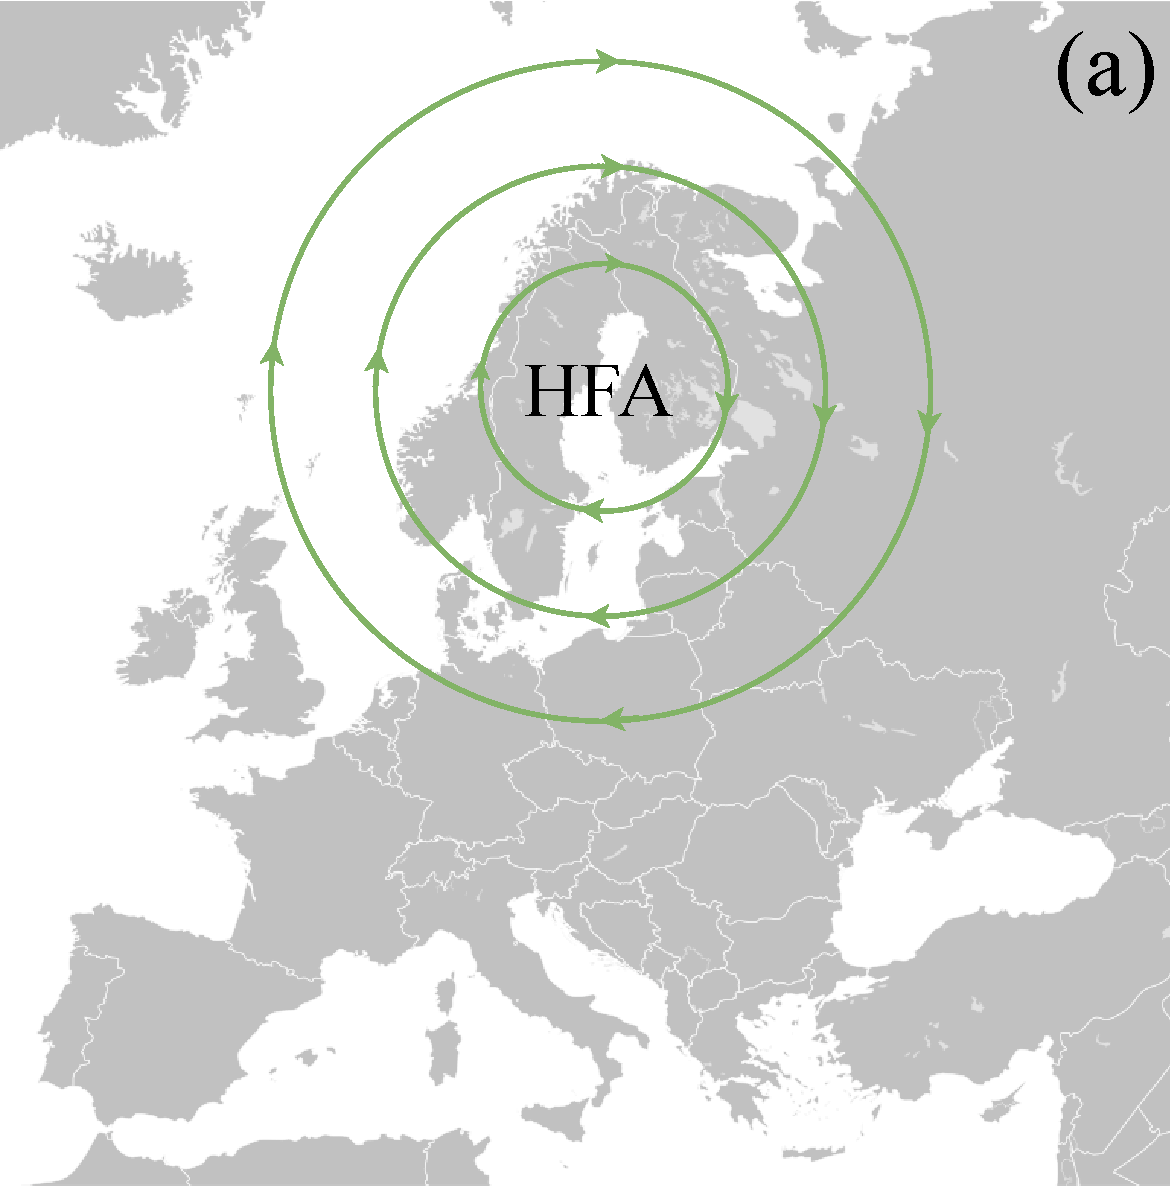
\includegraphics[width=\linewidth]{Figures/HFA.pdf}
    \end{minipage}
    \hfill
    \begin{minipage}{0.32\textwidth}
        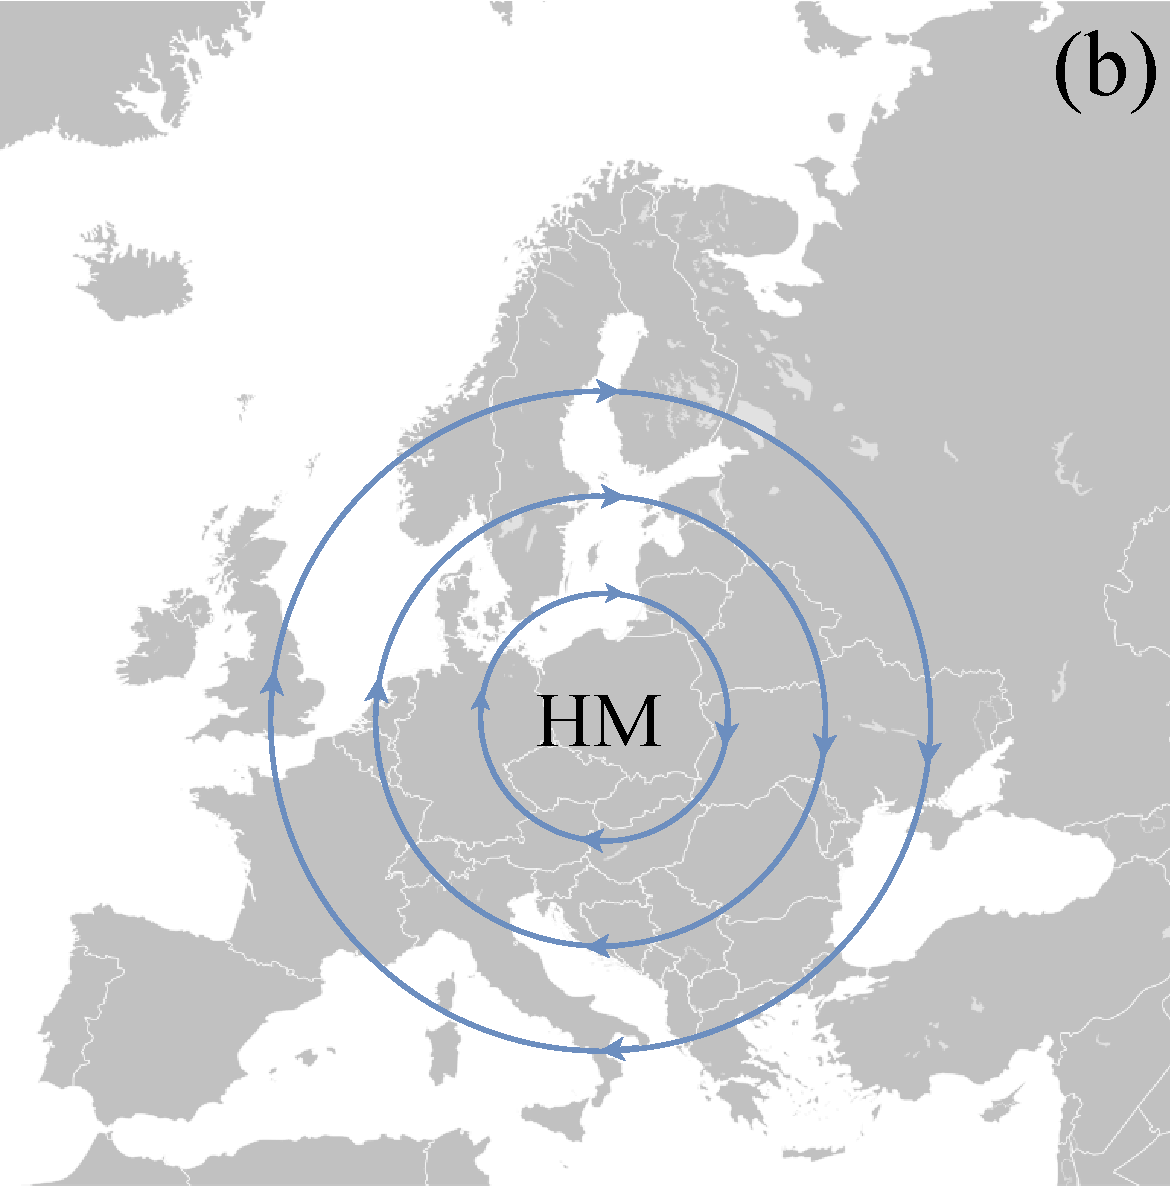
\includegraphics[width=\linewidth]{Figures/HM.pdf}
    \end{minipage}
    \hfill
    \begin{minipage}{0.32\textwidth}
        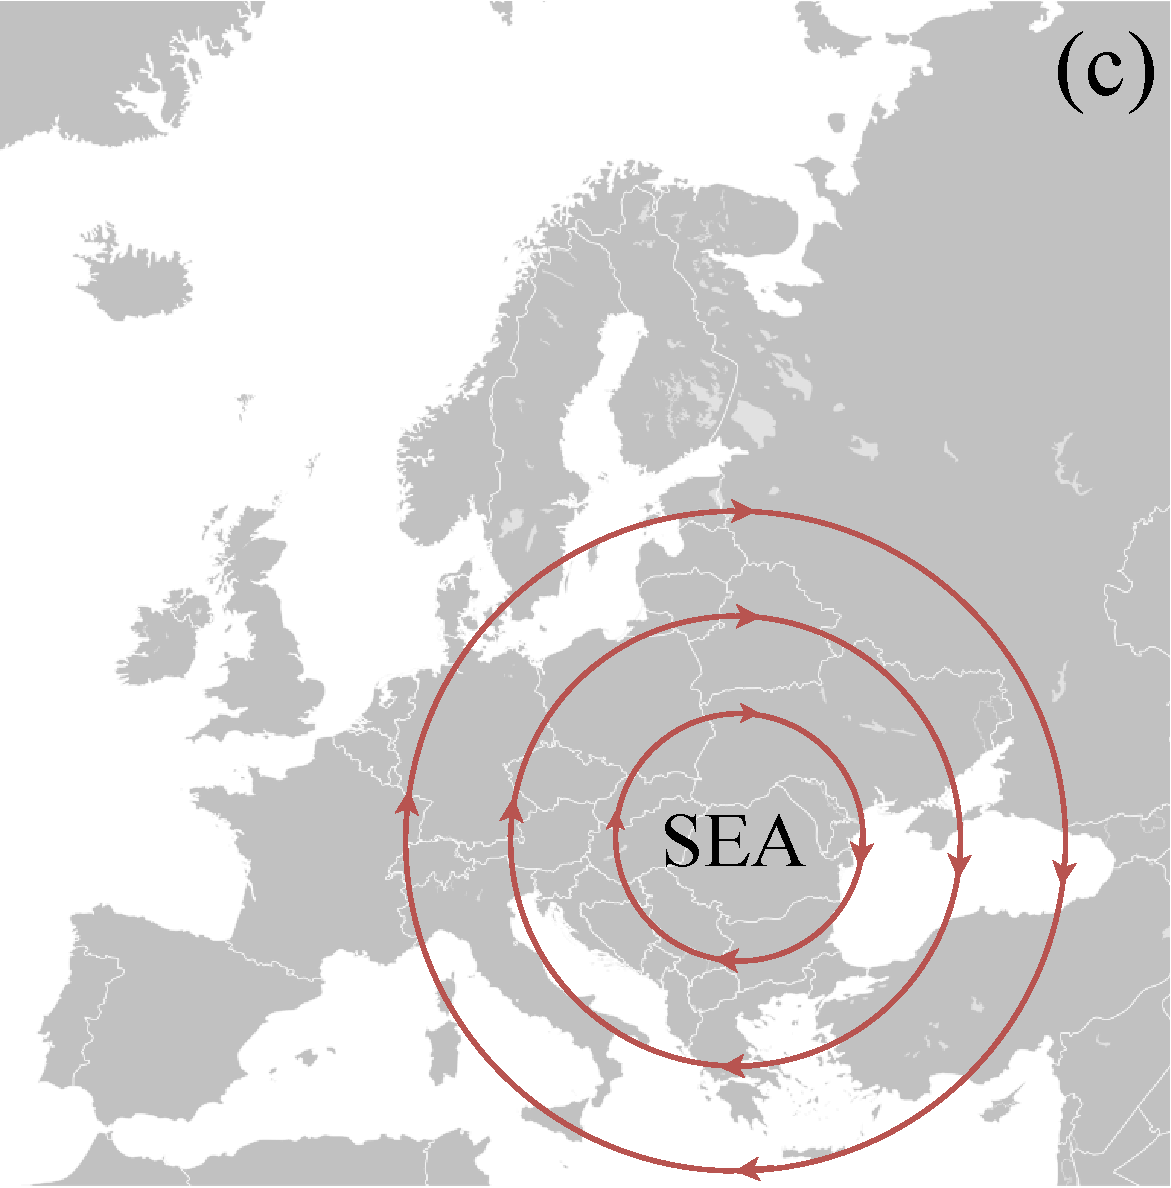
\includegraphics[width=\linewidth]{Figures/SEA.pdf}
    \end{minipage}
    \caption{These maps show the air movement during the HFA, HM, and SEA blocking events \cite{siglermarianBlankMapEurope2007}. The figures only show the general streamlines of the Brezowsky macrocirculation types, meaning that the real world anticyclones would not be perfectly circular.}
    \label{fig:map}
\end{figure}

\subsection{Aerosols}
Aerosols are liquid or solid particles suspended in the air. The concentration of aerosols in the air can be measured by the combined mass of the particulate matter per volume. However, it is important to specify which types of particles are being measured, where \PM(particulate matter with an aerodynamic diameter of \SI{2.5}{\micro\meter} or less) is a common choice because \PM is easy to measure. Furthermore \PM, like any other aerosol, impacts the health significantly and is able to be transported by the wind. Although aerosols can form naturally in the atmosphere, the primary sources in urban and suburban Europe include solid fuel combustion for domestic heating, industrial activities, and road transportation \cite{europeanenvironmentagencyEuropesAirQuality2024}. Particulate contributors to \PM include sulphur dioxide (SO\textsubscript{2}) and soot (black carbon), both originating from the burning of fossil fuels. The European Union set an annual mean limit for \PM concentrations at \SI{25}{\micro\gram\per\cubic\meter} in 2008, although the WHO suggested a much lower threshold of only \SI{5}{\micro\gram\per\cubic\meter} \cite{europeanenvironmentagencyEuropesAirQuality2024}. In 2022, the EU mean limit threshold was exceeded in several countries, including Croatia, Bosnia and Herzegovina, Italy, Poland, North Macedonia, and Türkiye \cite{europeanenvironmentagencyEuropesAirQuality2024}. 

Studies have demonstrated a correlation between elevated \PM concentrations and an increased risk of respiratory, cardiovascular, and cerebrovascular diseases, as well as diabetes \cite{sharmaHealthEffectsAssociated2020}. A Danish study on on \SI{49564}{} individuals between 1993 and 2015 showed that for every \SI{5}{\micro\gram\per
\m\cubed} increase in aerosol concentrations the hazard ratio increased by 1.29 \cite{hvidtfeldtLongtermResidentialExposure2019}. Thus, for every \SI{5}{\micro\gram\per
\m\cubed} increase in \PM the risk of dying from cardiovascular diseases increased by \SI{29}{\%}. Further studies on PM\textsubscript{10}, which is closely related to \PM, showed that in the age group of 75-84 mortality increased \SI{36}{\%} and \SI{106}{\%} in the age group 85+ during heath waves associated with high PM\textsubscript{10} concentrations \cite{analitisEffectsHeatWaves2014}.  


\subsubsection{Aerosol Concentrations During High-Pressure Blocking Events}
During a high-pressure blocking event the environmental lapse inversion, especially the subsidence inversion, close to the ground prohibits vertical air mixing during the atmospheric layers closest to the ground. If aerosols are produced at ground level during this high-pressure blocking event, this would imply that the aerosols would not disperse vertically, implying a higher concentration on the ground level. Thus, one would expect higher concentrations of \PM during high-pressure blocking events. Chinese studies have shown that the vertical dispersion of aerosols during high-pressure blocking events are inhibited, increasing the concentration of \PM in cities \cite{caiImpactBlockingStructure2020}.

Since aerosol emissions are particularly high in central European countries such as Poland, anticyclonic winds from the south and east from HFA, SEA, and HM are expected to increase \PM concentrations in southern Sweden \cite{europeanenvironmentagencyEuropesAirQuality2024}. These aerosols would be transported to southern Sweden via southerly to easterly winds during the anticyclone,  \autoref{fig:map}. If this occurs during a high-pressure blocking event, the aerosols may accumulate over the region while continuously being advected by southerly and easterly winds. A schematic figure showing why aerosols levels should increase in southern Sweden under high-pressure blocking events can be seen in \autoref{fig:Main_idea}. 

\vspace{1cm}

\begin{figure}[H]
    \centering
    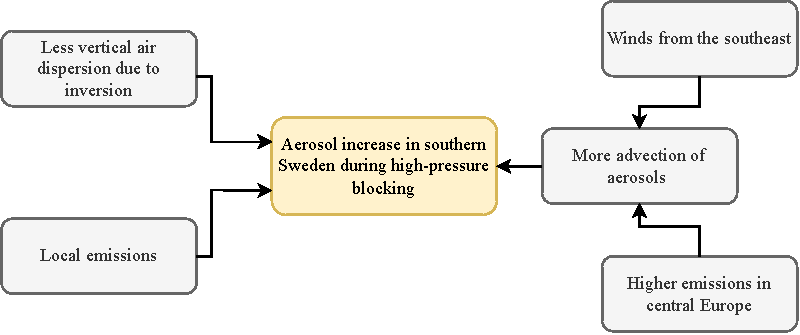
\includegraphics[width=0.8\textwidth]{Figures/Main_idea}
    \caption{This figure show why an aerosol increase should be observed during high-pressure blocking events in southern Sweden.}
    \label{fig:Main_idea}
\end{figure}


